\section{APR}

\begin{figure}[H]
\centering
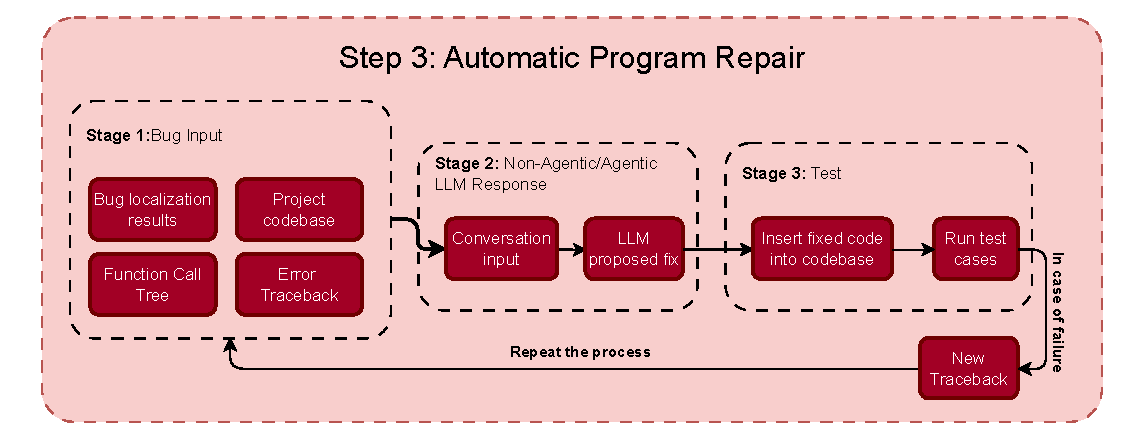
\includegraphics[width=1\columnwidth]{Figures/Step3_APR.drawio.pdf}
\caption{APR pipeline}
\label{fig:step2_bug_localization}
\end{figure}

LLMs are sensitive to the size and relevance of the input context. In practice, we found that providing entire source files—especially in legacy codebases where individual files may exceed 2,000 lines, substantially degrades the quality of repair suggestions. This is due to the dilution of relevant signal within overly broad inputs, often resulting in incoherent or incorrect fixes.

To address this limitation, we developed a targeted context-construction strategy that leverages both the error traceback and static code structure.

\subsection{Function Extraction from Error Traceback (Functional Call Tree)}

When a test case fails, we begin by analyzing the raw error traceback to identify all function calls that led to the failure. These functions are assumed to be highly relevant to the bug location. For each function, we retrieve the corresponding source code and extract any directly nested function calls within it (i.e., a call depth of 1). This process builds a partial call graph centered around the failing path.

\subsection{Reducing Context with Bug Localization (Not implemented yet)}
To further refine the set of candidate functions, we incorporate insights from the bug localization module. Functions that are deemed irrelevant based on localization confidence scores are discarded, ensuring that only high-signal code snippets are retained. The resulting context—comprising the error traceback and filtered function bodies is then provided to the LLM.

\subsection{Iterative Repair and Retesting}
The LLM generates a proposed fix based on the curated input. This fix is inserted directly into the codebase at the appropriate location. The modified code is then recompiled and retested. If the test fails again, the process is repeated using the new error traceback, allowing for up to three iterations. If no successful fix is found after three attempts, the process is terminated.

\subsection{Results}

\begin{table}[H]
\centering
\begin{tabularx}{\textwidth}{lccc}
\toprule
\textbf{Project} & \textbf{First Pass} & \textbf{Second Pass} & \textbf{Third Pass} \\
\midrule
youtube-dl & 48.64\% & 62.16\% & 72.22\% \\
\bottomrule
\end{tabularx}
\caption{Bug repair accuracy across multiple passes for the  projects}
\label{tab:apr_projects}
\end{table}
